Our proposed segmentation algorithm was applied to the Salinas dataset and its performance was evaluated using established evaluation metrics like Overall Accuracy (OA), Average Segmentation Accuracy (ASA), and Intersection over Union (IoU) for individual classes. This evaluation will allow us to assess the effectiveness of our algorithm in segmenting the Salinas scene, particularly focusing on its ability to accurately identify and delineate the various material classes present within the dataset.

For Salinas-A, prior knowledge about the scene confirms the aim is to segment the image into $n_e = 6$ segments corresponding to the following vegetation classifications in the image. One important note is that Label 10 is commonly understood to be incorrectly label, this is due to the presence of two differing spectral signatures in endmember. As such, the aim is to then segement the image in $n_e = 7$ segments corresponding to this new spectral distinction within Label 10. For the sake of evaluation against the known labels, segmentations created by the algorithm within this region will be joined into one label.
\begin{table}[H]
    % \caption{Groundtruth classes for the Salinas-A scene and their respective samples number}
    \centering
    \label{tab:salinas_classes}
    \begin{tabular}{|c|c|c|}
    \hline
    \textbf{Label} & \textbf{Class} & \textbf{Samples} \\
    \hline
    1 & Broccoli green weeds 1 & 391 \\
    10 & Corn-senesced green weeds & 1343 \\
    11 &Lettuce romaine 4wk & 616 \\
    12 & Lettuce romaine 5wk & 1525 \\
    13 & Lettuce romaine 6wk & 674 \\
    14 &Lettuce romaine 7wk & 799 \\
    \hline
    \end{tabular}
    \caption{Groundtruth classes for the Salinas-A scene and their respective samples number}
\end{table}
\begin{figure}[h]
    \centering
    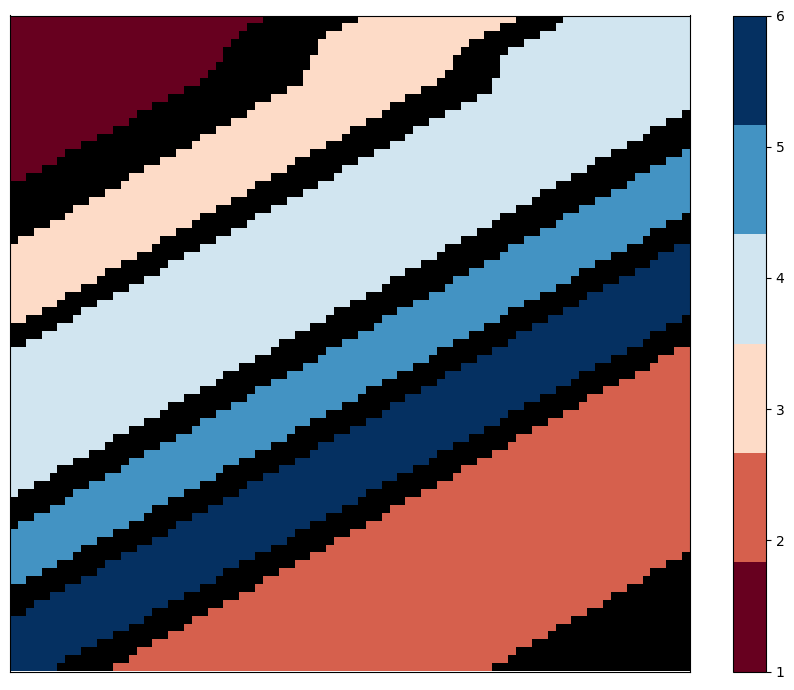
\includegraphics[width=10cm]{salinas-a-error.png}  % Adjust width and filename
    \caption{Salinas-A Gound Truth Labels}
    \label{salina-a}  % Optional label for referencing
  \end{figure}
\clearpage

Using an initial selection of $n_s = 420$ superpixels with shape parameter $m=2$ and unmixing parameters $\mu = 1$ and $\beta = 0.0025$, a grid search was applied to $\sigma$ and $\kappa$ such that $\sigma \in [0.1, 0.001]$ and $\kappa \in [15, 40]$, to which $\sigma = 0.0025$ and $\kappa = 20$ produced the most optimal results with an overall accuracy of $0.993$.
\begin{figure}[H]
    \centering
    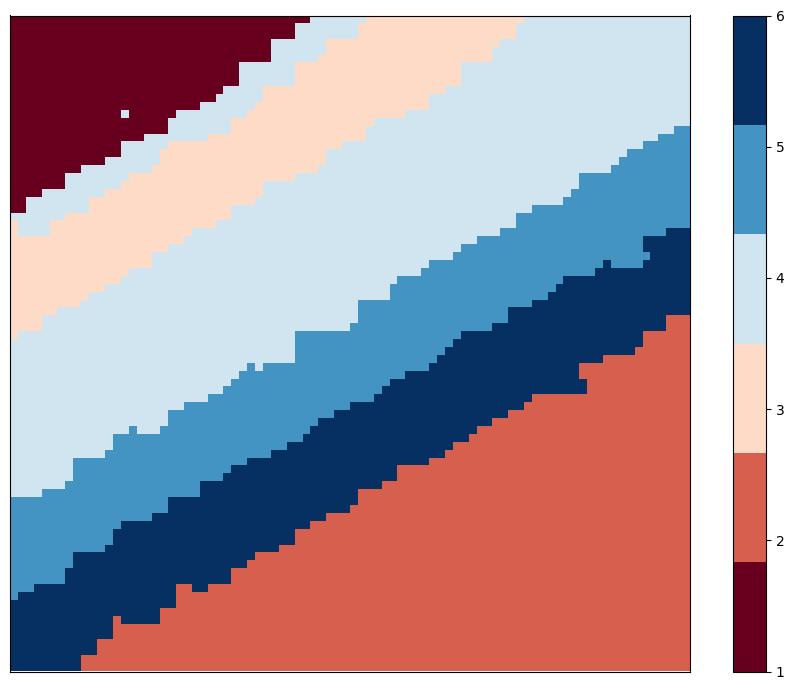
\includegraphics[width=10cm]{salinas-a-labelled.png}  % Adjust width and filename
    \caption{Salinas-A Algorithm Results}
    \label{salina-a-results}  % Optional label for referencing
\end{figure}

In the case of this specific segmentation, predicted segments $5$ and $10$ were combined to match with the comparison to label $13$. The algorithm itself performs well across all classes, with high individual segment accuracy scores aswell as IoU scores, demonstrating it's ability to perform segmentation in scenarios where similar spectral features are shared among materials and materials span across the image.
\begin{table}[H]
    \centering
    \label{tab:salinas_cfm}
    \begin{tabular}{|c|cccccc|c|c|}
        \hline
         & \textbf{1} & \textbf{10} & \textbf{11} & \textbf{12} & \textbf{13} & \textbf{14} & \textbf{Accuracy} & \textbf{IoU} \\ \hline
        1      &  390    &  0    &  0    &  10    &  0    &  0    &  0.997 & 0.997  \\ 
        10      &  0    & 1343  &  0    &  0    &  0    &  0     &  1.000   & 0.987\\ 
        11      &  0    &  0    &  598  &  180   &  0    &  0    &  0.971  & 0.971\\ 
        12      &  0    &  0    &  0    & 1525  &  0    &  0    &  1.000  & 0.988\\ 
        13      &  0    &  0    &  0    &  0    &  671  &  30    &  0.996  & 0.996\\ 
        14      &  0    &  180   &  0    &  0    &  0    &  781  &  0.977  & 0.974\\ \hline
    \end{tabular}
    \caption{Pixel-wise Confusion Matrix (Vertical: Actual, Horizontal: Predicted)}
\end{table}

Salinas-B is a simpler segmentation case, prior knowledge about the scene confirms the aim is to segment the image into $n_e = 5$ segments corresponding to the following vegetation classifications in the image.
\begin{table}[H]
    % \caption{Groundtruth classes for the Salinas-A scene and their respective samples number}
    \centering
    \label{tab:salinas_b_classes}
    \begin{tabular}{|c|c|c|}
    \hline
    \textbf{Label} & \textbf{Class} & \textbf{Samples} \\
    \hline
    4 & Fallow Rough Plow & 490 \\
    5 & Fallow Smooth & 989 \\
    6 & Stubble & 1627 \\
    7 & Celery & 1127 \\
    15 & Vinyard Untrained  & 2891 \\
    \hline
    \end{tabular}
    \caption{Groundtruth classes for the Salinas-B scene and their respective samples number}
\end{table}
\begin{figure}[H]
    \centering
    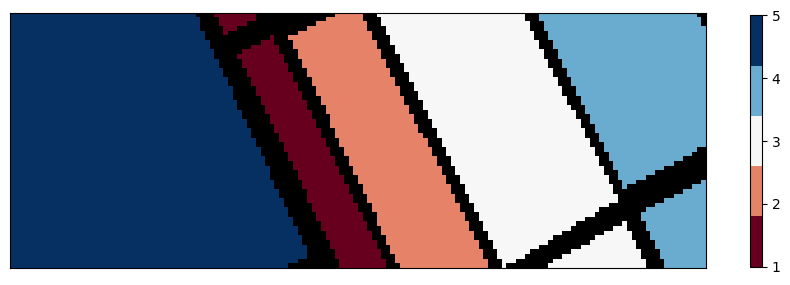
\includegraphics[width=10cm]{salinas-b-gt.png}  % Adjust width and filename
    \caption{Salinas-B Gound Truth Labels}
    \label{salina-b}  % Optional label for referencing
\end{figure}


Using an initial selection of $n_s = 330$ superpixels with shape parameter $m=2$ and unmixing parameters $\mu = 1$ and $\beta = 0.0025$, a grid search was applied to $\sigma$ and $\kappa$ such that $\sigma \in [0.1, 0.001]$ and $\kappa \in [15, 40]$, to which $\sigma = 0.005$ and $\kappa = 10$ produced the most optimal results with an overall accuracy of $0.998$. 
\begin{figure}[H]
    \centering
    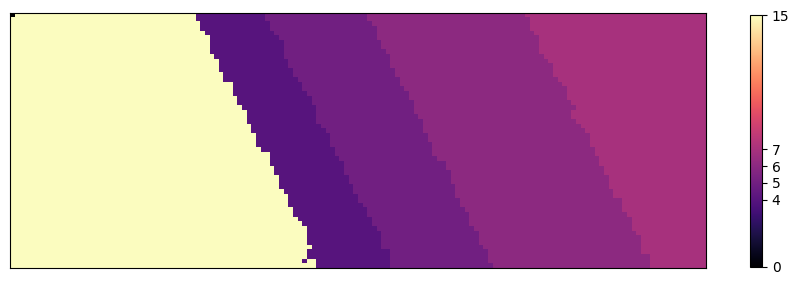
\includegraphics[width=10cm]{salinas-b-labelled.png}  % Adjust width and filename
    \caption{Salinas-B Algorithm Results}
    \label{salina-b-results}  % Optional label for referencing
\end{figure}
\begin{table}[H]
    \centering
    \label{tab:salinas_b_cfm}
    \begin{tabular}{|c|ccccc|c|c|}
        \hline
         & \textbf{4} & \textbf{5} & \textbf{6} & \textbf{7} & \textbf{15} & \textbf{Accuracy} & \textbf{IoU} \\ \hline
        4      &  490    &  0    &  0    &  0        &  0    &  1.00 & 0.992  \\ 
        5      &  0    & 989  &  0    &  0        &  0    &  1.000   & 1.00\\ 
        6      &  0    &  0    &  1621  &  6       &  0    &  0.996  & 0.996\\ 
        7      &  0    &  0    &  0    & 1127    &  0    &  1.000  & 0.995\\ 
        15      &  4   &  0    &  0    &  0      &  2887    &  0.999  & 0.999\\ \hline
    \end{tabular}
    \caption{Pixel-wise Confusion Matrix (Vertical: Actual, Horizontal: Predicted)}
\end{table}
Again, the algorithm itself performs well across all classes, with high individual segment accuracy scores aswell as IoU scores, demonstrating it's ability to perform segmentation in scenarios where similar spectral features are shared among materials and materials span across the image.

    


